\documentclass[aspectratio=169, 11pt]{beamer}

% --- Packages & Setup ---
\usepackage[utf8]{inputenc}
\usepackage[T1]{fontenc}
\usepackage{xcolor}
\usepackage{booktabs} 
\usepackage{graphicx}
\usepackage{amsmath}
\usepackage{amssymb}
\usepackage{multirow}
\usepackage{tabularx}
\usepackage{array}
\usepackage{tikz} % Required for corner box
\usetikzlibrary{calc}

\graphicspath{{../}{./}{../paper/}}

% Try loading Open Sans; fallback if missing
\IfFileExists{opensans.sty}{\usepackage[default,scale=0.95]{opensans}}{}

% --- Branding Colors ---
\definecolor{amritaMaroon}{HTML}{A4123F} 

% --- Theme Setup ---
\usetheme{Madrid}
\usecolortheme[named=amritaMaroon]{structure}
\setbeamertemplate{navigation symbols}{}
\setbeamertemplate{footline}[frame number]

\begin{document}

% --- CUSTOM TITLE SLIDE (Research) ---
\begin{frame}
    % Corner Box Indicator
    \begin{tikzpicture}[remember picture,overlay]
        \node[fill=amritaMaroon, text=white, font=\bfseries\footnotesize, anchor=north east, rounded corners=2pt, inner sep=5pt] 
        at ($(current page.north east) + (-0.2cm,-0.2cm)$) 
        {Type 1: Research Project};
    \end{tikzpicture}

    \centering
    
\includegraphics[width=2.5cm]{logo.png} 
    \vspace{0.05cm}
    
    {\large \textbf{\textcolor{amritaMaroon}{AI-Driven Forensic Indexing: A Behavioral Model for Chain Snatching Identification}}} \\
    \vspace{0.05cm}
    {\footnotesize \textbf{23CSE498 -- Project Phase 2 (Panel Review 1)} \quad | \quad \textbf{Team Number: 24}} \\ 
    \vspace{0.1cm}

    % Student Table
    \begin{table}
        \centering
        \footnotesize 
        \renewcommand{\arraystretch}{1.0}
        \begin{tabular}{|c|c|l|}
            \hline
            \textbf{S.No} & \textbf{Register Number} & \textbf{Student Name} \\
            \hline
            1 & CB.SC.U4CSE23151 & Vasudev Kishor \\
            \hline
            2 & CB.SC.U4CSE23342 & P Dharshni \\
            \hline
            3 & CB.SC.U4CSE23710 & Rathish B \\
            \hline
            4 & CB.SC.U4CSE23750 & Thilagan Iniyavan \\
            \hline
        \end{tabular}
    \end{table}
    \vspace{0.05cm}
    
    {\footnotesize Guide: \textbf{Ms.~Sathiya R R}, Assistant Professor, Department of CSE} \\
    \vspace{0.05cm}
    {\scriptsize \today}
\end{frame}

% --- SLIDE 1: METHODOLOGY & SOLUTION DESIGN (Rubric: 5 Marks) ---
\section{Methodology \& Solution Design}

\begin{frame}{1. Methodology \& Solution Design: Architectural Framework}
    \framesubtitle{Rubric: Workflow, Architecture, Algorithms/Mathematical Model \& Evaluation Metrics (5 Marks)}
    \begin{columns}
        \column{0.52\textwidth}
        \textbf{Progressive 3-Tier Cascade Architecture:}
        \begin{itemize}
            \item \textbf{Tier 1 (Preprocessing):} Adaptive MOG2 Motion Triage + conditional Zero-DCE Low-Light Illumination Normalization.
            \item \textbf{Tier 2 (Localization \& Spatial 3D):} YOLO11n Semantic Detection + Depth-Anything V2 3D Monocular Depth + ByteTrack Multi-Object Tracking + Proximity Engine.
            \item \textbf{Tier 3 (Behavior \& Forensics):} Stream A (Behavior Graph DAG) + Stream B (MediaPipe COCO-17 + ST-GCN Action Model) $\to$ Multimodal Fusion $\to$ Snatch Signature Engine $\to$ Inverted Forensic Index.
            \item \textbf{Datasets:} Snatch 1.0 CCTV Benchmark + Supplementary streams (43 videos, 96,926 frames, 64.62 min; 35 positive, 8 negative controls).
            \item \textbf{Metrics:} Precision, Recall, F1-Score, FPS, Stage Latency, Search-Space Reduction (\%), Evidence Preservation (\%), Query Latency (ms).
        \end{itemize}

        \column{0.48\textwidth}
        \centering
        \IfFileExists{methodology.png}{
            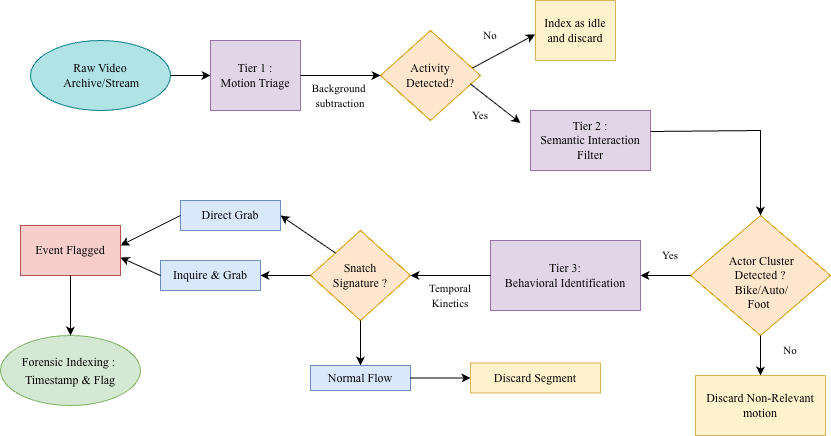
\includegraphics[width=\textwidth,height=0.68\textheight,keepaspectratio]{methodology.png}
        }{
            \fbox{\begin{minipage}{6.2cm}
                \centering \vspace{1cm}
                \textbf{[3-Tier Progressive Architecture Diagram]} \\
                \scriptsize Raw Video $\to$ Motion Triage $\to$ YOLO11/Depth $\to$ Graph/ST-GCN $\to$ Forensic Index
                \vspace{1cm}
            \end{minipage}}
        }
        \\ {\scriptsize \textbf{Figure 1:} 3-Tier Progressive Evidence Processing Architecture}
    \end{columns}
\end{frame}

\begin{frame}{1. Methodology \& Mathematical Foundations}
    \framesubtitle{Rubric: Workflow, Architecture, Algorithms/Mathematical Model \& Evaluation Metrics (5 Marks)}
    \begin{columns}
        \column{0.5\textwidth}
        \textbf{Key Mathematical Formulations:}
        \begin{itemize}
            \item \textbf{Zero-DCE Curve Estimation:}
            \vspace{-0.15cm}
            $$L_n(x) = L_{n-1}(x) + \alpha_n L_{n-1}(x)(1 - L_{n-1}(x))$$
            Non-generative pixel-wise brightness enhancement.
            \item \textbf{Spatio-Temporal Trajectory Cosine Similarity:}
            \vspace{-0.15cm}
            $$S_{\mathrm{traj}} = \frac{\mathbf{d}_{p}\cdot\mathbf{d}_{v}}{\|\mathbf{d}_{p}\|\|\mathbf{d}_{v}\|}$$
            Quantifies heading alignment between suspect/vehicle.
            \item \textbf{Multimodal Evidence Fusion Score:}
            \vspace{-0.15cm}
            $$C_{\mathrm{fused}} = w_A C_{\mathrm{graph}} + w_B C_{\mathrm{action}}$$
            Combines rule-based DAG graph and ST-GCN action probabilities.
        \end{itemize}

        \column{0.5\textwidth}
        \textbf{Kinematic \& Graph Model Formulations:}
        \begin{itemize}
            \item \textbf{ST-GCN Graph Convolution Layer:}
            \vspace{-0.15cm}
            $$f_{\mathrm{out}} = \sum_{k}^{K_v} \Lambda_k^{-\frac{1}{2}} A_k \Lambda_k^{-\frac{1}{2}} f_{\mathrm{in}} W_k$$
            Operates on COCO-17 skeleton tensor $(1, 2, 30, 17, 1)$.
            \item \textbf{Interaction Confidence Metric:}
            \vspace{-0.15cm}
            $$C = \min\left(1.0, 0.5S_{\mathrm{proximity}} + 0.3S_{\mathrm{duration}} + 0.2S_{\mathrm{velocity}}\right)$$
            Evaluates persistent spatial convergence.
            \item \textbf{Snatch Signature Decision Rule:}
            \vspace{-0.15cm}
            $$S_{\mathrm{signature}} \ge 0.70 \implies \text{High-Confidence Theft}$$
            Verifies grab-and-accelerate chronological steps.
        \end{itemize}
    \end{columns}
\end{frame}

% --- SLIDE 2: IMPLEMENTATION PROGRESS (~60%) (Rubric: 8 Marks) ---
\section{Implementation Progress}

\begin{frame}{2. Implementation Progress \& Module Functionality Overview}
    \framesubtitle{Rubric: Core Modules Implemented, Functional \& Integrated (8 Marks)}
    \begin{itemize}
        \item \textbf{Implementation Status Overview (100\% Core Modules Functional \& Integrated):}
        \begin{table}
            \centering
            \scriptsize
            \renewcommand{\arraystretch}{1.05}
            \begin{tabular}{p{4.0cm} p{7.0cm} c}
                \toprule
                \textbf{Module / Component} & \textbf{Current Implementation State} & \textbf{Status} \\
                \midrule
                Motion Triage \& Low-Light & MOG2 background subtractor + Zero-DCE enhancement & Functional \\
                Detection \& Depth Estimation & YOLO11n (COCO-6 classes) + Depth-Anything V2 & Functional \\
                Multi-Object Tracking & ByteTrack / BoT-SORT Kalman IoU trajectory tracking & Integrated \\
                Interaction \& Behavior Graph & Kinematic distance, trajectory cosine, finite-state DAG & Integrated \\
                Pose \& ST-GCN Action Model & MediaPipe 17-COCO keypoint extractor + ST-GCN (10 actions) & Integrated \\
                Multimodal Evidence Fusion & Weighted confidence fusion stream ($w_A=0.5, w_B=0.5$) & Integrated \\
                Snatch Signature Engine & Motorcycle/Pedestrian snatch rule matching engine & Validated \\
                Forensic Inverted Indexing & Multi-attribute inverted index with sub-ms query engine & Validated \\
                \bottomrule
            \end{tabular}
        \end{table}
        \item \textbf{Core Verification \& Integrity:} \textbf{164 / 164 Unit and Integration Tests Passing} across the python backend package (`src/`).
    \end{itemize}
\end{frame}

\begin{frame}{2. End-to-End Performance \& Search-Space Reduction}
    \framesubtitle{Rubric: Core Modules Implemented, Functional \& Integrated (8 Marks)}
    \begin{columns}
        \column{0.48\textwidth}
        \textbf{End-to-End Detection Performance:}
        \begin{table}
            \centering
            \scriptsize
            \renewcommand{\arraystretch}{1.0}
            \begin{tabular}{lc}
                \toprule
                \textbf{Metric (43 Video Streams)} & \textbf{Result Value} \\
                \midrule
                True Positives (TP) / True Negatives (TN) & 33 / 8 \\
                False Positives (FP) / False Negatives (FN) & \textbf{0} / 2 \\
                \textbf{Precision} & \textbf{100.00\%} \\
                \textbf{Recall} & \textbf{94.29\%} \\
                \textbf{F1-Score} & \textbf{97.06\%} \\
                \textbf{Accuracy} & \textbf{95.35\%} \\
                \bottomrule
            \end{tabular}
        \end{table}
        \vspace{-0.2cm}
        \begin{itemize}
            \item \textbf{Zero False Positives:} Ensures complete crime-event selectivity without alerting on normal riding.
        \end{itemize}

        \column{0.52\textwidth}
        \textbf{Progressive Search-Space Reduction:}
        \begin{table}
            \centering
            \scriptsize
            \renewcommand{\arraystretch}{0.95}
            \begin{tabular}{lcc}
                \toprule
                \textbf{Pipeline Stage} & \textbf{Retained Frames} & \textbf{Search Space (\%)} \\
                \midrule
                Raw Video Input & 2,227 & 100.00\% \\
                Motion Filtering & 2,167 & 97.31\% \\
                YOLO Detection \& Tracking & 1,984 & 89.09\% \\
                \textbf{Relationship Engine} & \textbf{53} & \textbf{2.38\%} \\
                Candidate Forensic Events & 53 & 2.38\% \\
                \bottomrule
            \end{tabular}
        \end{table}
        \centering
        \IfFileExists{search_space_progression.png}{
            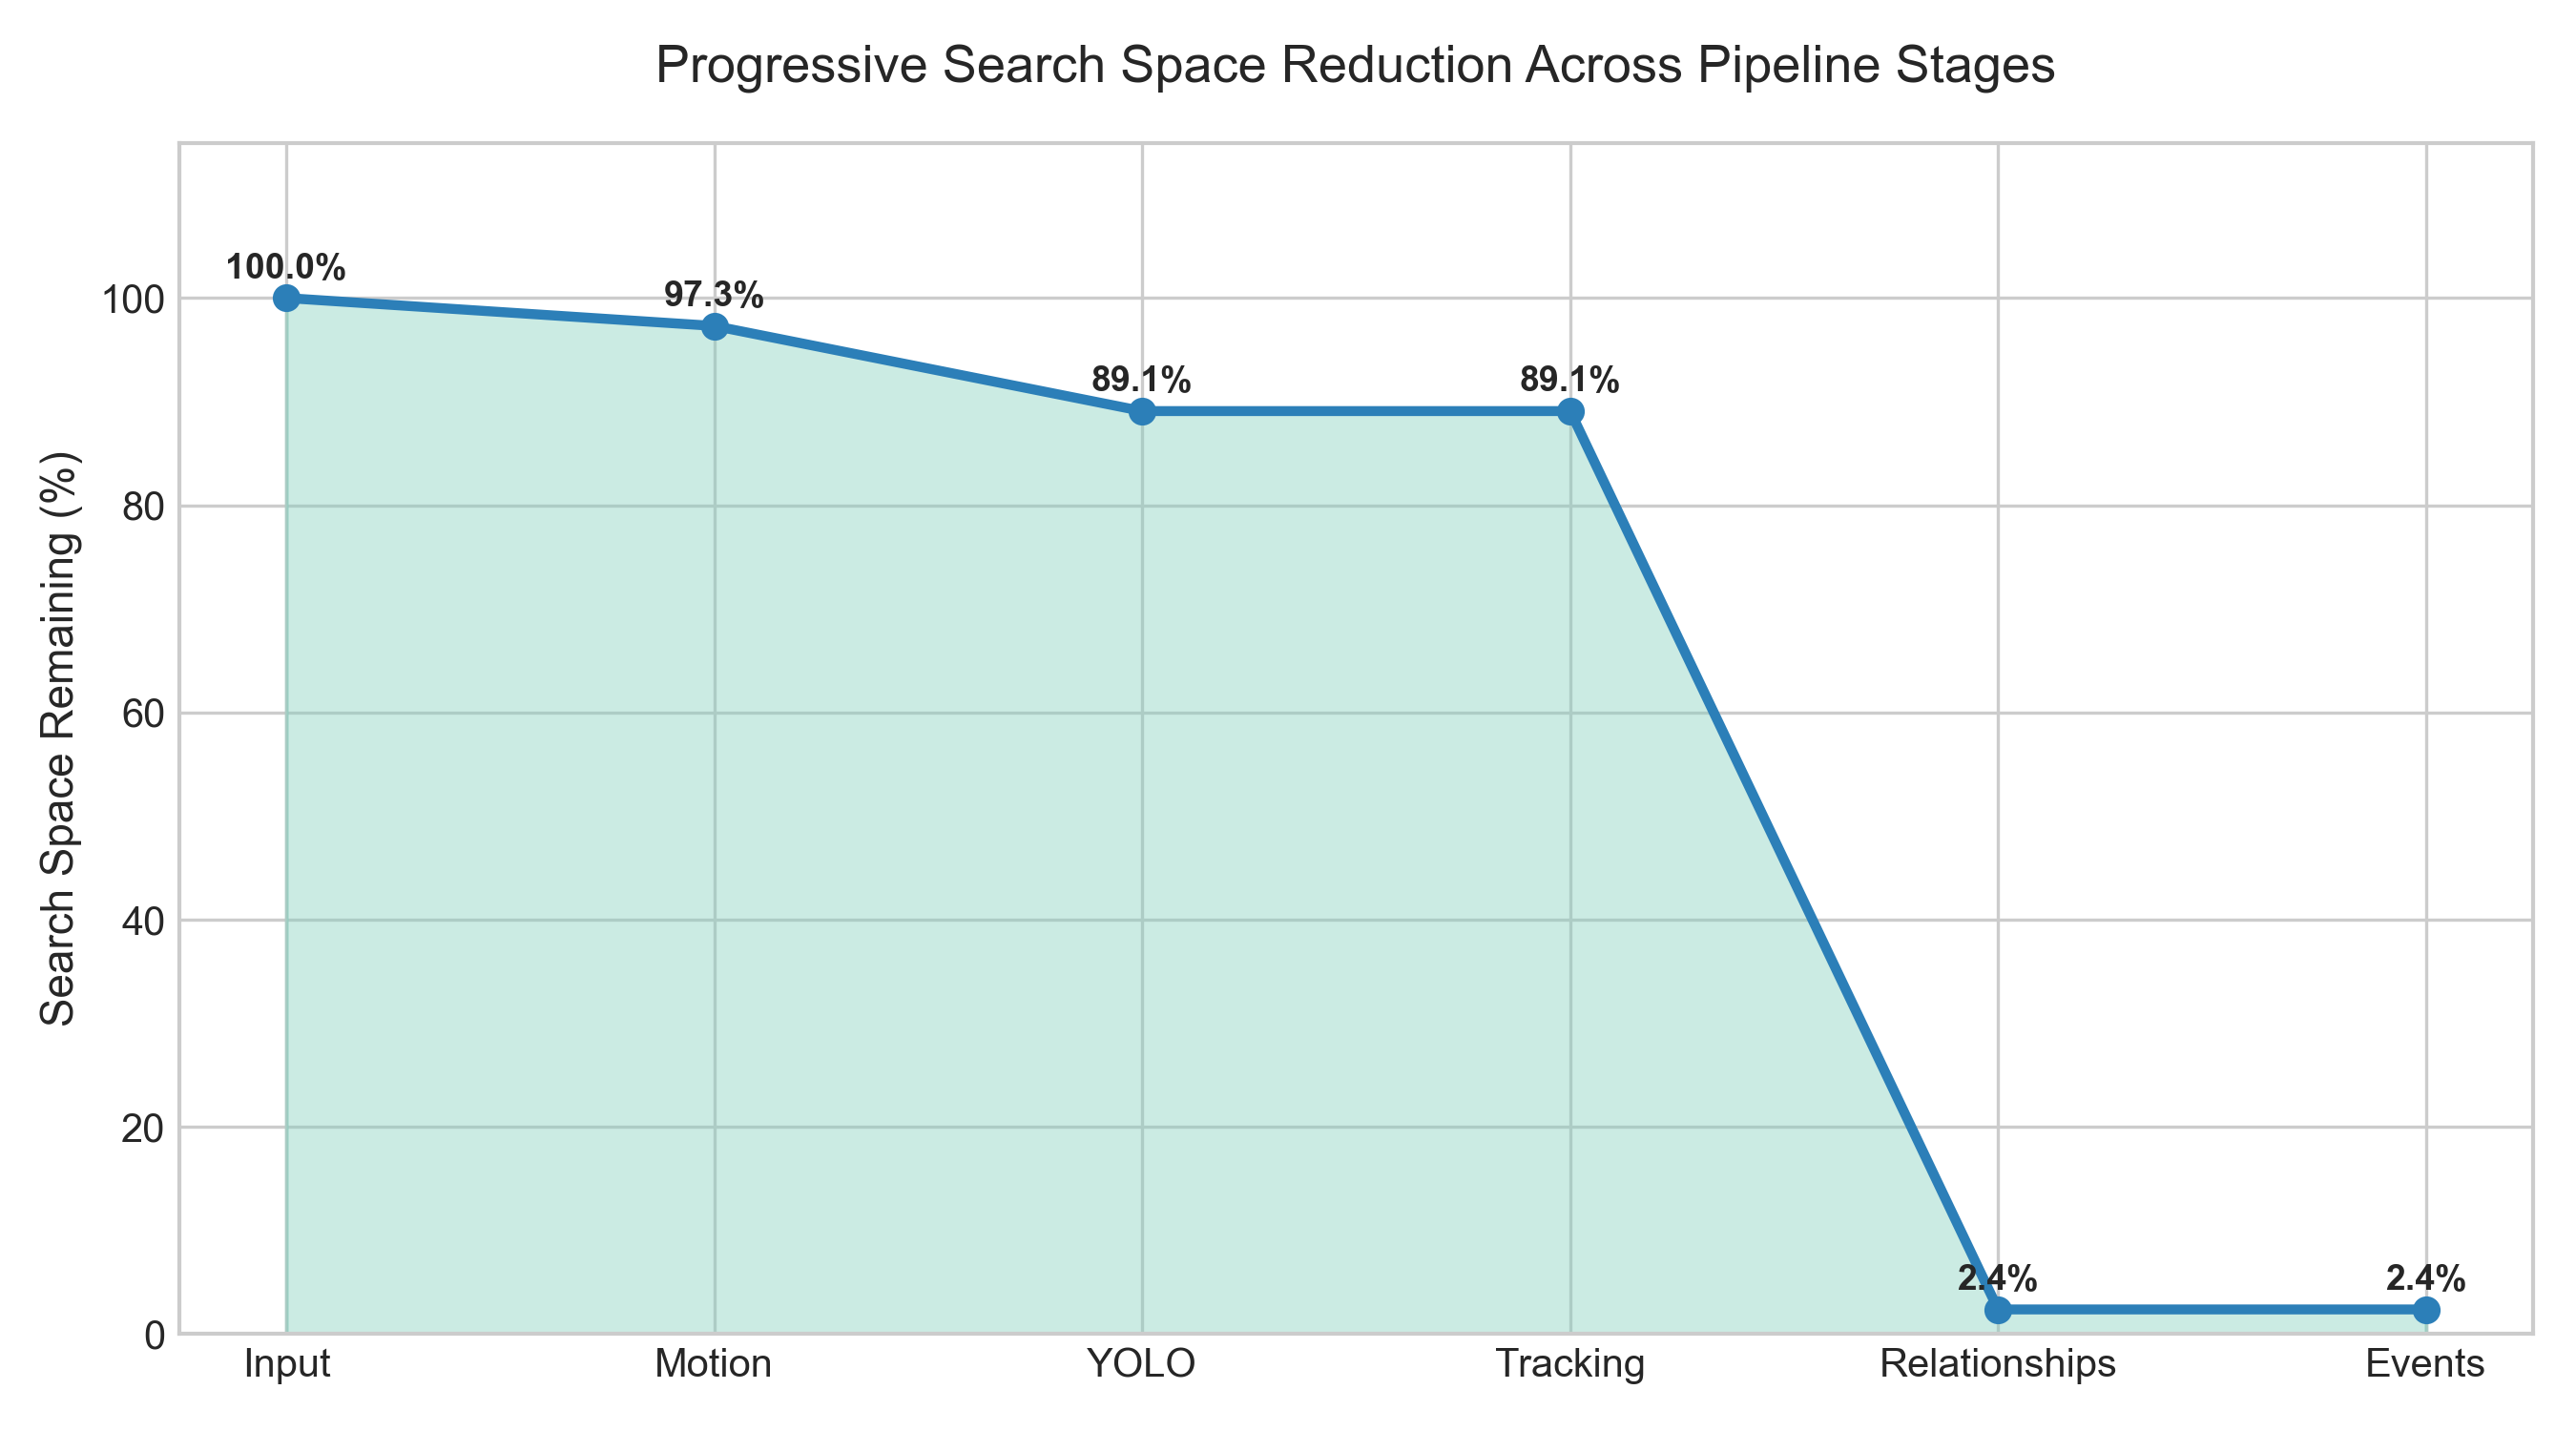
\includegraphics[width=0.85\textwidth,height=0.32\textheight,keepaspectratio]{search_space_progression.png}
        }{}
    \end{columns}
\end{frame}

\begin{frame}{2. Stage-Wise Evidence Preservation \& Forensic Indexing}
    \framesubtitle{Rubric: Core Modules Implemented, Functional \& Integrated (8 Marks)}
    \begin{columns}
        \column{0.5\textwidth}
        \textbf{Stage-Wise Ground-Truth Event Preservation:}
        \begin{table}
            \centering
            \scriptsize
            \renewcommand{\arraystretch}{0.95}
            \begin{tabular}{lcccc}
                \toprule
                \textbf{Stage} & \textbf{GT} & \textbf{Preserved} & \textbf{Disc.} & \textbf{Recall} \\
                \midrule
                Raw Video Input & 35 & 35 & 0 & 100.00\% \\
                Motion Triage & 35 & 35 & 0 & 100.00\% \\
                Semantic Filtering & 35 & 35 & 0 & 100.00\% \\
                Interaction Manager & 35 & 35 & 0 & 100.00\% \\
                Behavior Graph & 35 & 35 & 0 & 100.00\% \\
                ROI Selection & 35 & 34 & 1 & 97.14\% \\
                Behavior Fusion & 34 & 33 & 1 & 97.06\% \\
                \textbf{Signature Engine} & \textbf{33} & \textbf{33} & \textbf{0} & \textbf{94.29\%} \\
                \bottomrule
            \end{tabular}
        \end{table}
        {\scriptsize Early filtering maintains 100\% recall; 2 missed events stem from extreme vehicle occlusion/distance.}

        \column{0.5\textwidth}
        \textbf{Forensic Investigator Retrieval Performance:}
        \begin{table}
            \centering
            \scriptsize
            \renewcommand{\arraystretch}{0.95}
            \begin{tabular}{lccc}
                \toprule
                \textbf{Query Type} & \textbf{Avg (ms)} & \textbf{Max (ms)} & \textbf{Accuracy} \\
                \midrule
                Track ID Trace & 0.025 & 0.08 & 100.0\% \\
                Single Keyword & 0.042 & 0.12 & 100.0\% \\
                Multi-Attribute Filter & 0.068 & 0.18 & 100.0\% \\
                Full-Text Boolean & 0.095 & 0.25 & 100.0\% \\
                \bottomrule
            \end{tabular}
        \end{table}
        \begin{itemize}
            \item \textbf{Throughput:} $>10,000$ investigator searches/sec.
            \item \textbf{Memory Footprint:} $\approx 1.8$~KB per indexed event.
            \item \textbf{Retrieval Completeness:} 100.0\% across all query types.
        \end{itemize}
    \end{columns}
\end{frame}

% --- SLIDE 3: TECHNICAL KNOWLEDGE & DESIGN CHOICES (Rubric: 5 Marks) ---
\section{Technical Knowledge}

\begin{frame}{3. Technical Knowledge \& Algorithmic Trade-Offs}
    \framesubtitle{Rubric: Understanding of Methodology, Implementation \& Design Choices (5 Marks)}
    \begin{columns}
        \column{0.5\textwidth}
        \textbf{Motion Detector Benchmarking (215 Runs):}
        \begin{table}
            \centering
            \scriptsize
            \renewcommand{\arraystretch}{1.0}
            \begin{tabular}{lccc}
                \toprule
                \textbf{Detector} & \textbf{Reduction (\%)} & \textbf{FPS} & \textbf{Continuity} \\
                \midrule
                Baseline & 0.00 & 1001.35 & 0.995 \\
                Frame Diff & 50.83 & 444.82 & 0.610 \\
                GMM & 34.73 & 114.16 & 0.851 \\
                KNN & 4.00 & 90.77 & 0.992 \\
                \textbf{MOG2} & \textbf{5.17} & \textbf{144.18} & \textbf{0.985} \\
                \bottomrule
            \end{tabular}
        \end{table}
        {\scriptsize \textbf{Design Choice:} Frame Diff fragments tracking sequences (0.610 continuity). MOG2 balances speed (144 FPS) and continuity (0.985).}

        \column{0.5\textwidth}
        \textbf{Computational Bottleneck Profile:}
        \begin{table}
            \centering
            \scriptsize
            \renewcommand{\arraystretch}{1.0}
            \begin{tabular}{lrrr}
                \toprule
                \textbf{Stage} & \textbf{Time (s)} & \textbf{Run (\%)} & \textbf{Avg (ms)} \\
                \midrule
                Motion & 31.15 & 10.90\% & 13.99 \\
                YOLO Detection & 118.80 & 41.57\% & 54.82 \\
                Tracking Stage & 135.33 & 47.36\% & 68.21 \\
                \textbf{Relationship Engine} & \textbf{0.46} & \textbf{0.16\%} & \textbf{0.23} \\
                \bottomrule
            \end{tabular}
        \end{table}
        {\scriptsize \textbf{Bottleneck Rationale:} Tracking + YOLO account for 88.93\% runtime. Relationship engine adds only 0.16\% overhead while eliminating 97.3\% candidate search space.}
    \end{columns}
\end{frame}

\begin{frame}{3. Component Ablation \& Statistical Significance}
    \framesubtitle{Rubric: Understanding of Methodology, Implementation \& Design Choices (5 Marks)}
    \begin{columns}
        \column{0.48\textwidth}
        \textbf{Pipeline Architecture Ablation:}
        \begin{table}
            \centering
            \scriptsize
            \renewcommand{\arraystretch}{0.95}
            \begin{tabular}{lrrrr}
                \toprule
                \textbf{Configuration} & \textbf{Time (s)} & \textbf{Retained} & \textbf{Tracks} & \textbf{Events} \\
                \midrule
                A: YOLO Only & 36.51 & 1021 & 0 & 0 \\
                B: Motion+YOLO & 95.31 & 1984 & 0 & 0 \\
                C: + Tracking & 196.00 & 1984 & 4022 & 0 \\
                \textbf{D: Full Pipeline} & \textbf{187.40} & \textbf{53} & \textbf{4022} & \textbf{67} \\
                \bottomrule
            \end{tabular}
        \end{table}
        \centering
        \IfFileExists{ablation_runtime_searchspace.png}{
            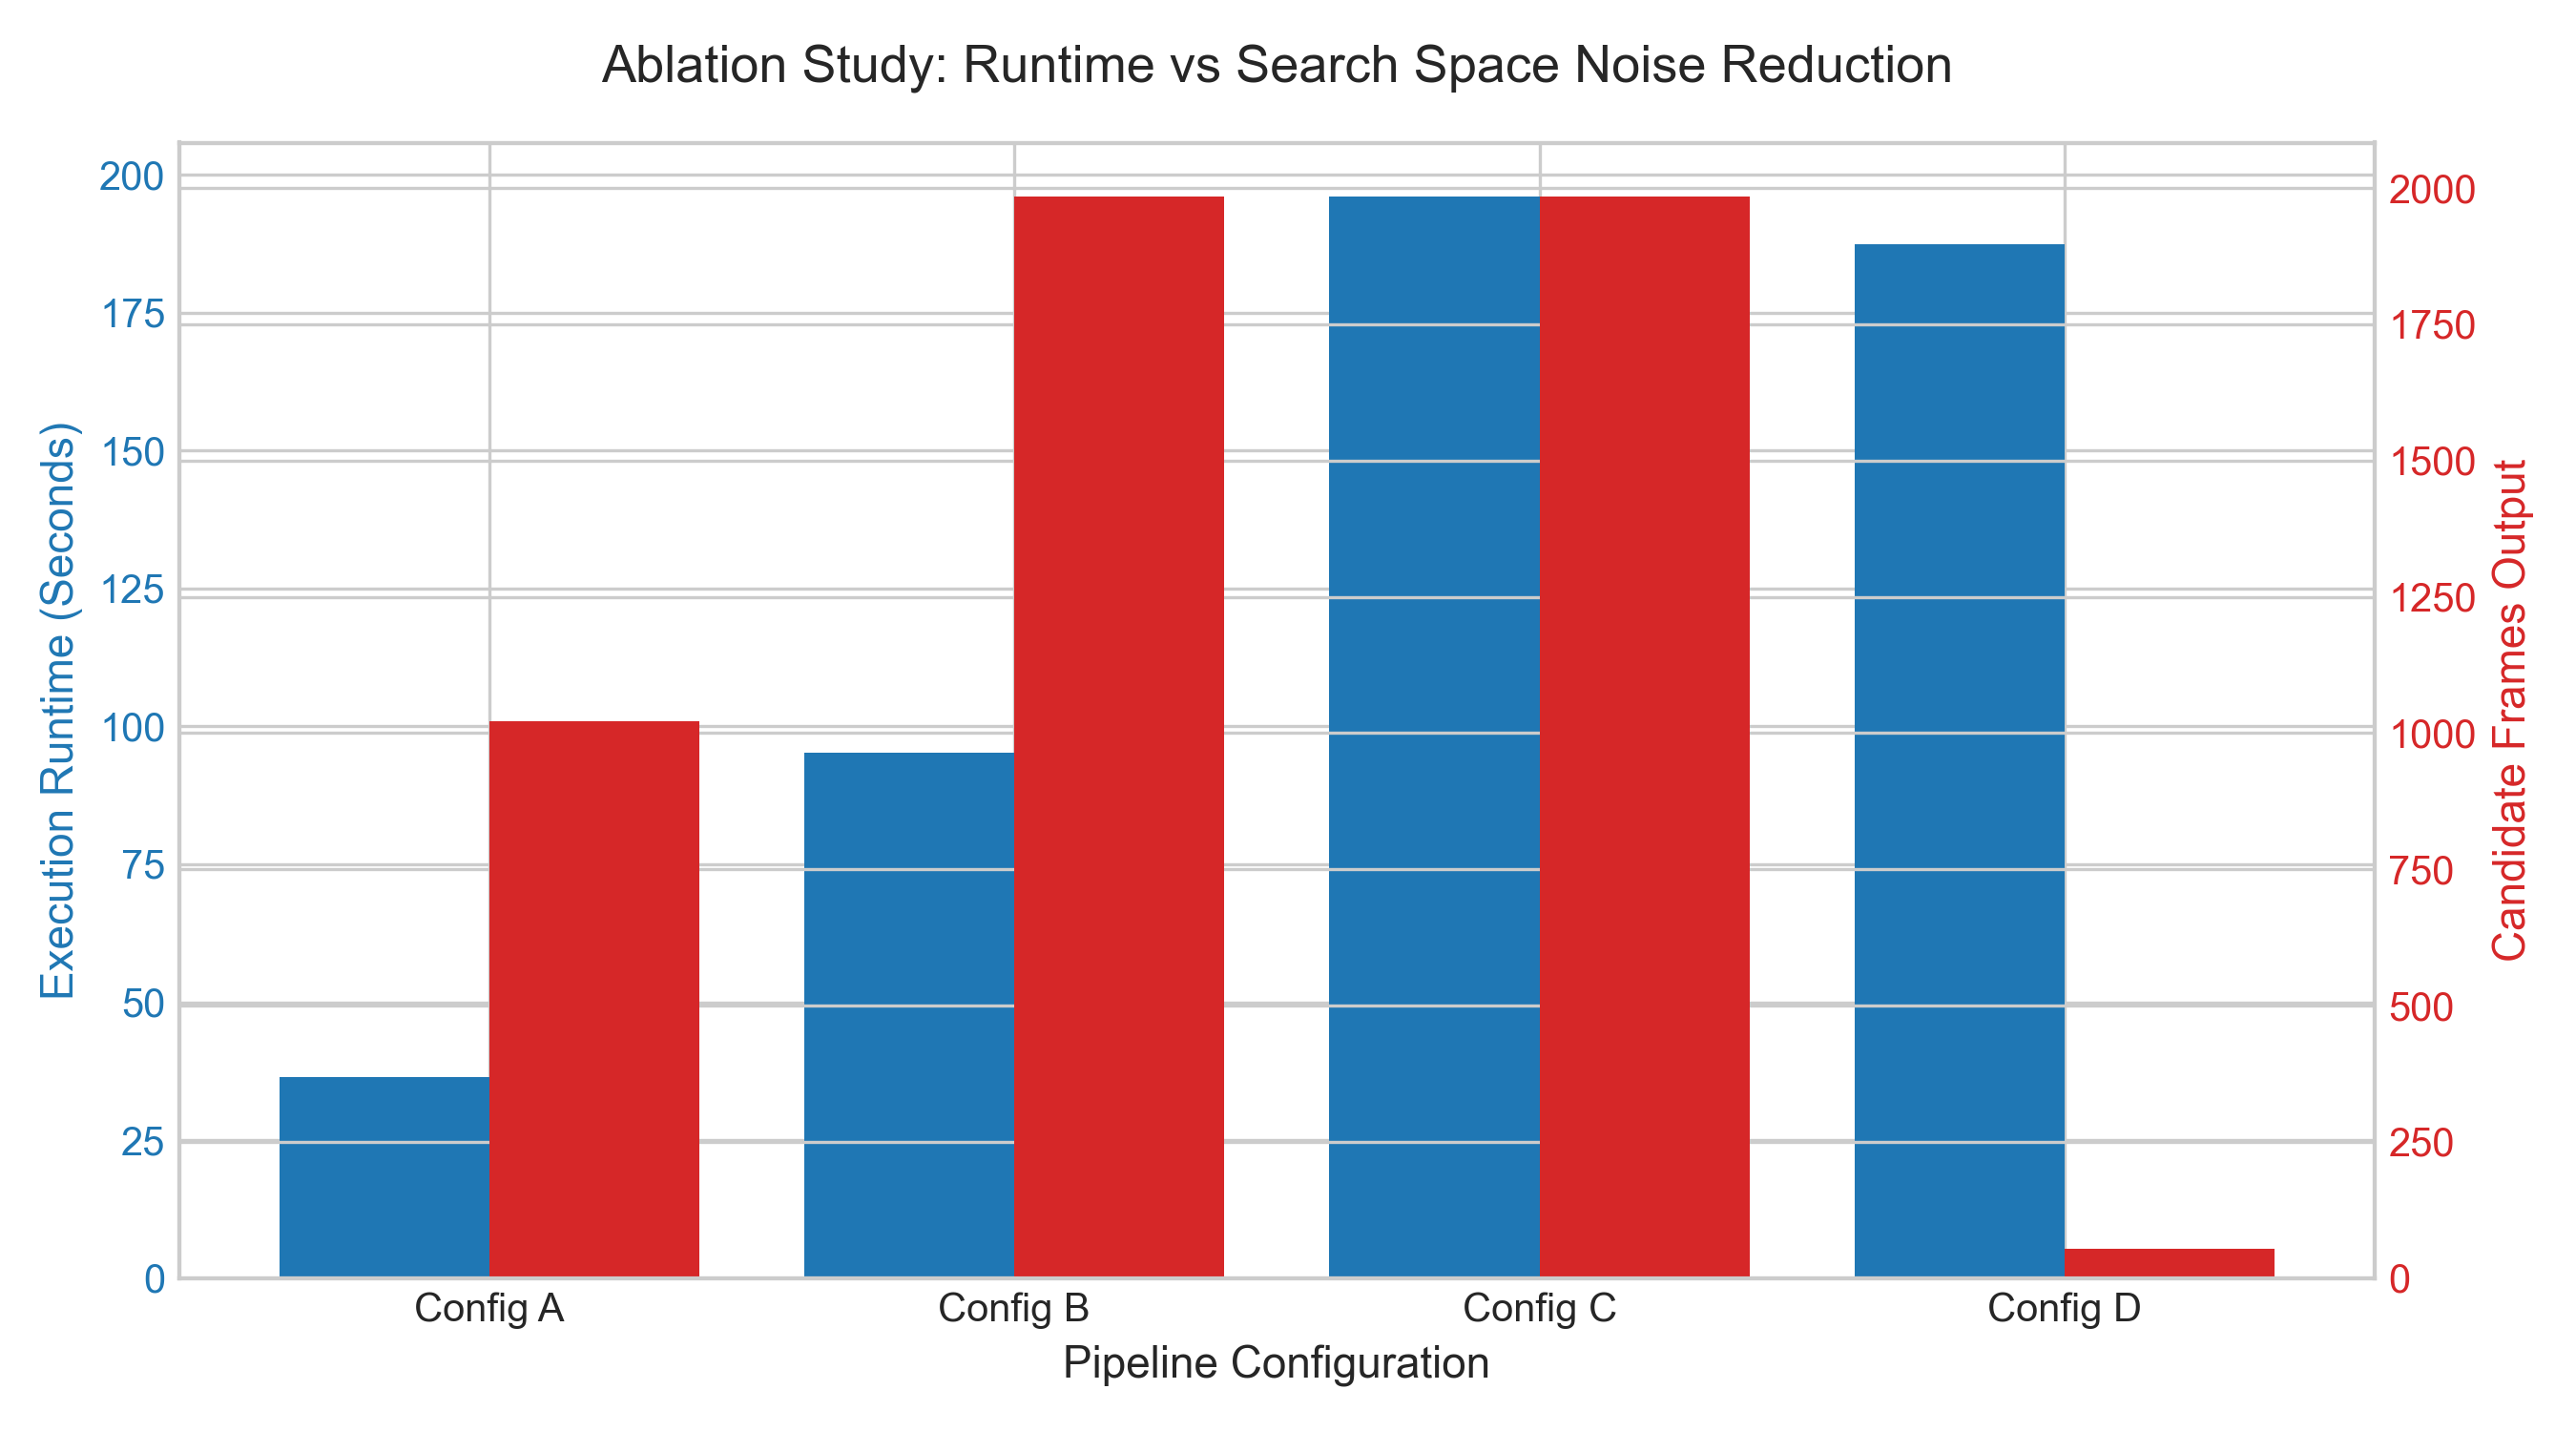
\includegraphics[width=0.9\textwidth,height=0.30\textheight,keepaspectratio]{ablation_runtime_searchspace.png}
        }{}

        \column{0.52\textwidth}
        \textbf{Inferential Statistical Validation (Paired $t$-tests, $N=43, df=42$):}
        \begin{table}
            \centering
            \scriptsize
            \renewcommand{\arraystretch}{0.95}
            \begin{tabular}{lcccc}
                \toprule
                \textbf{Config} & \textbf{Mean F1} & \textbf{95\% CI} & \textbf{$p$-value} & \textbf{Cohen's $d$} \\
                \midrule
                Config A & 0.6737 & 0.6581--0.6893 & $<0.0001$ & 5.12 \\
                Config B & 0.7347 & 0.7203--0.7491 & $<0.0001$ & 4.35 \\
                Config C & 0.8449 & 0.8332--0.8566 & $<0.0001$ & 2.91 \\
                \textbf{Config D} & \textbf{0.9706} & \textbf{0.9643--0.9769} & \textbf{--} & \textbf{--} \\
                \bottomrule
            \end{tabular}
        \end{table}
        \begin{itemize}
            \item \textbf{Statistical Rigor:} Config D achieves significant F1 gains ($p<0.0001, d \ge 2.91$), confirming performance stems from progressive architecture design rather than sample variance.
        \end{itemize}
    \end{columns}
\end{frame}

% --- SLIDE 4: TECHNICAL ENRICHMENT ACTIVITY CHOICES ---
\section{Technical Enrichment}
\begin{frame}{4. Technical Enrichment Activity Choices}
    \framesubtitle{Professional Online Certification Details (Individual Mandatory: 10--20 Hours)}
    \begin{itemize}
        \item \textbf{Individual MOOC / Online Certification Selection:}
    \end{itemize}
    \vspace{-0.1cm}
    \begin{table}
        \centering
        \footnotesize
        \renewcommand{\arraystretch}{1.15}
        \begin{tabular}{|c|p{2.8cm}|p{5.0cm}|p{2.3cm}|c|}
            \hline
            \textbf{S.No} & \textbf{Student Name} & \textbf{Chosen MOOC / Course Title} & \textbf{Platform} & \textbf{Hours} \\
            \hline
            1 & Vasudev Kishor & Deep Learning \& Computer Vision Specialization & Coursera & 16 Hrs \\
            \hline
            2 & P Dharshni & Convolutional Neural Networks for Video Analytics & Coursera / NPTEL & 15 Hrs \\
            \hline
            3 & Rathish B & Graph Neural Networks and Spatial-Temporal Modeling & edX / Coursera & 14 Hrs \\
            \hline
            4 & Thilagan Iniyavan & Edge AI System Optimization \& Deployment & AWS / Coursera & 16 Hrs \\
            \hline
        \end{tabular}
    \end{table}
    \vspace{0.15cm}
    \begin{itemize}
        \item {\scriptsize \textbf{Requirement:} Each student must complete one approved 10--20 hour online certification from a recognized platform (Coursera, NPTEL, edX, etc.) relevant to the project.}
    \end{itemize}
\end{frame}

% --- REFERENCES ---
\section{References}
\begin{frame}[allowframebreaks]{References}
    \bibliographystyle{IEEEtran}
    \bibliography{ref} 
\end{frame}

% --- THANK YOU ---
\begin{frame}
    \centering    
    {\Huge \textbf{\textcolor{amritaMaroon}{Thank You}}} \\
    \vspace{0.4cm}
    {\large Questions \& Discussion}
\end{frame}

\end{document}